\section{Experiments}

We evaluate progressive networks across three different RL domains.
First, we consider synthetic versions of Pong,
altered to have visual or control-level
similarities. Next, we experiment broadly with random
sequences of Atari games and perform a feature-level transfer analysis.
Lastly, we demonstrate performance
on a set of 3D maze games. Fig.~\ref{fig:datasets} shows examples from selected tasks.

\begin{figure}[h]
\centering
\subfloat[Pong variants]{
\begin{tabular}{cc}
  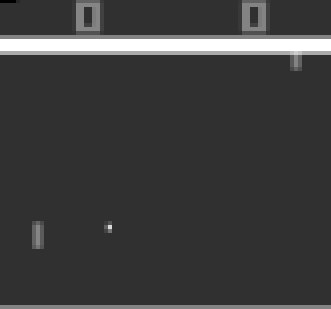
\includegraphics[width=.09\textwidth]{figures/pong_plain.png}&
  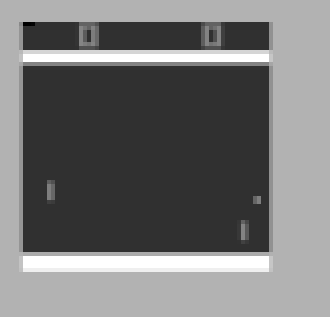
\includegraphics[width=.09\textwidth]{figures/pong_zoom.png}\\
  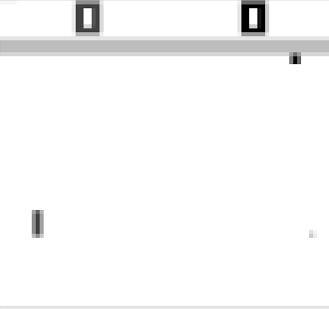
\includegraphics[width=.09\textwidth]{figures/pong_white.png}&
  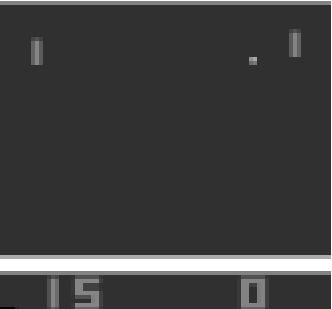
\includegraphics[width=.09\textwidth]{figures/pong_hvflip.png}
\end{tabular}
}
\subfloat[Labyrinth games]{
\begin{tabular}{cc}
  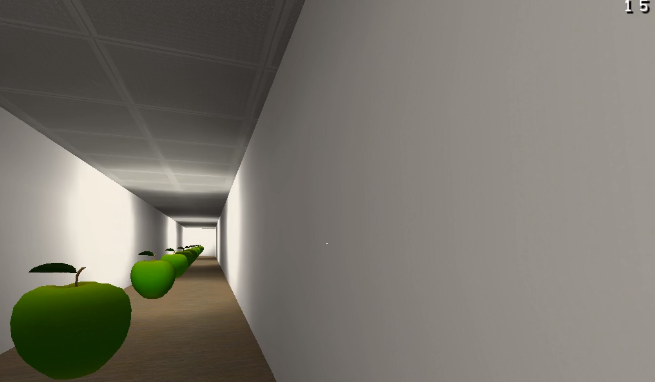
\includegraphics[width=.15\textwidth]{figures/seek_track_01.png}&
  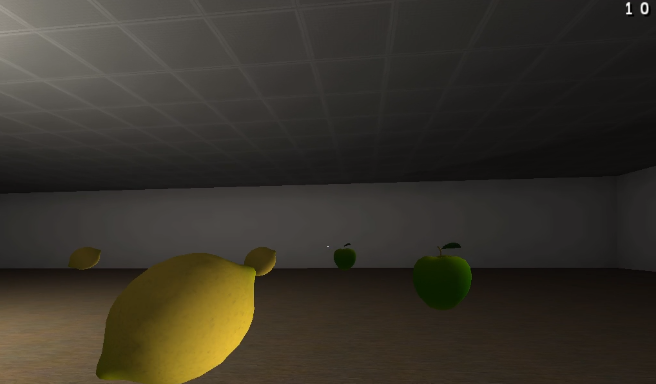
\includegraphics[width=.15\textwidth]{figures/seekavoid_arena_01.png}\\
  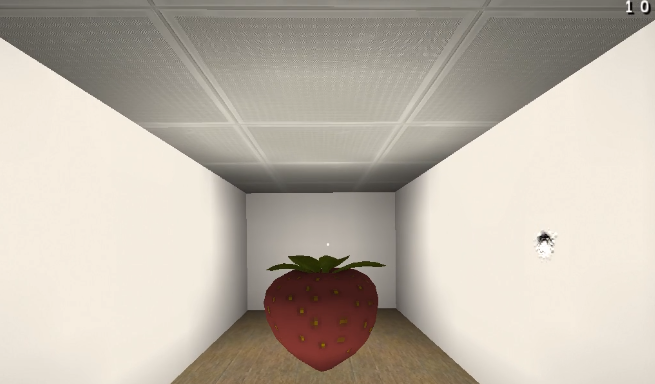
\includegraphics[width=.15\textwidth]{figures/seek_track_02.png}&
  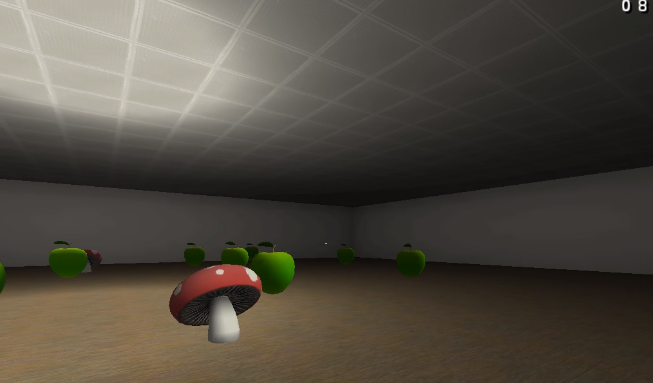
\includegraphics[width=.15\textwidth]{figures/seekavoid_arena_02.png}
\end{tabular}
}
\subfloat[Atari games]{
\begin{tabular}{cc}
  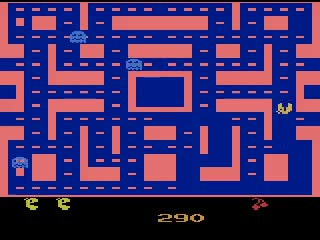
\includegraphics[width=.12\textwidth]{figures/pacman.jpg}&
  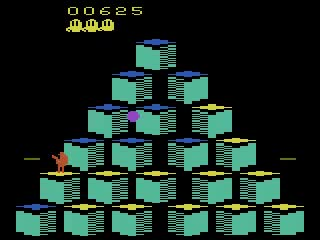
\includegraphics[width=.12\textwidth]{figures/qbert.jpg}\\
  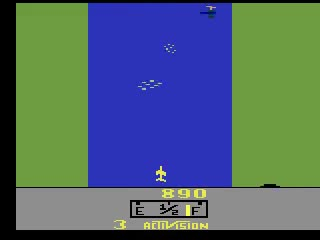
\includegraphics[width=.12\textwidth]{figures/rraid.jpg}&
  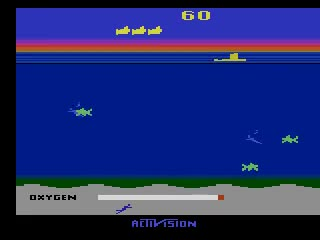
\includegraphics[width=.12\textwidth]{figures/seaquest.jpg}
\end{tabular}
}
\hfill
\caption{Samples from different task domains: (a) Pong variants include flipped, noisy, scaled, and recoloured transforms; (b) Labyrinth is a set of 3D maze games with diverse level maps and diverse positive and negative reward items; (c) Atari games offer a more challenging setting for transfer.}
\label{fig:datasets}
\end{figure}

\subsection{Setup}

We rely on the Async Advantage Actor-Critic (A3C) framework introduced in
\citep{mnih2016a3c}.  Compared to DQN \citep{mnih-dqn-2015}, the model simultaneously learns
a policy and a value function
for predicting expected future rewards. A3C is trained on CPU using multiple threads
and has been shown to converge faster than DQN on GPU. This made it
a more natural fit for the
large amount of sequential experiments required for this work.

We report results by averaging the top 3 out of 25 jobs, each having
different seeds and random hyper-parameter sampling. Performance is evaluated
by measuring the area under the learning curve (average score per
episode during training), rather than final score. The \emph{transfer score}
is then defined as the relative performance of an architecture compared with
a single column baseline, trained only on the target task (baseline 1). We present transfer
score curves for selected source-target games, and summarize all such pairs in
\emph{transfer matrices}.
Models and baselines we consider are illustrated in Figure \ref{fig:baselines}.
Details of the experimental setup are provided in section 3 of the Appendix.

\begin{figure}[h]
  \centering
    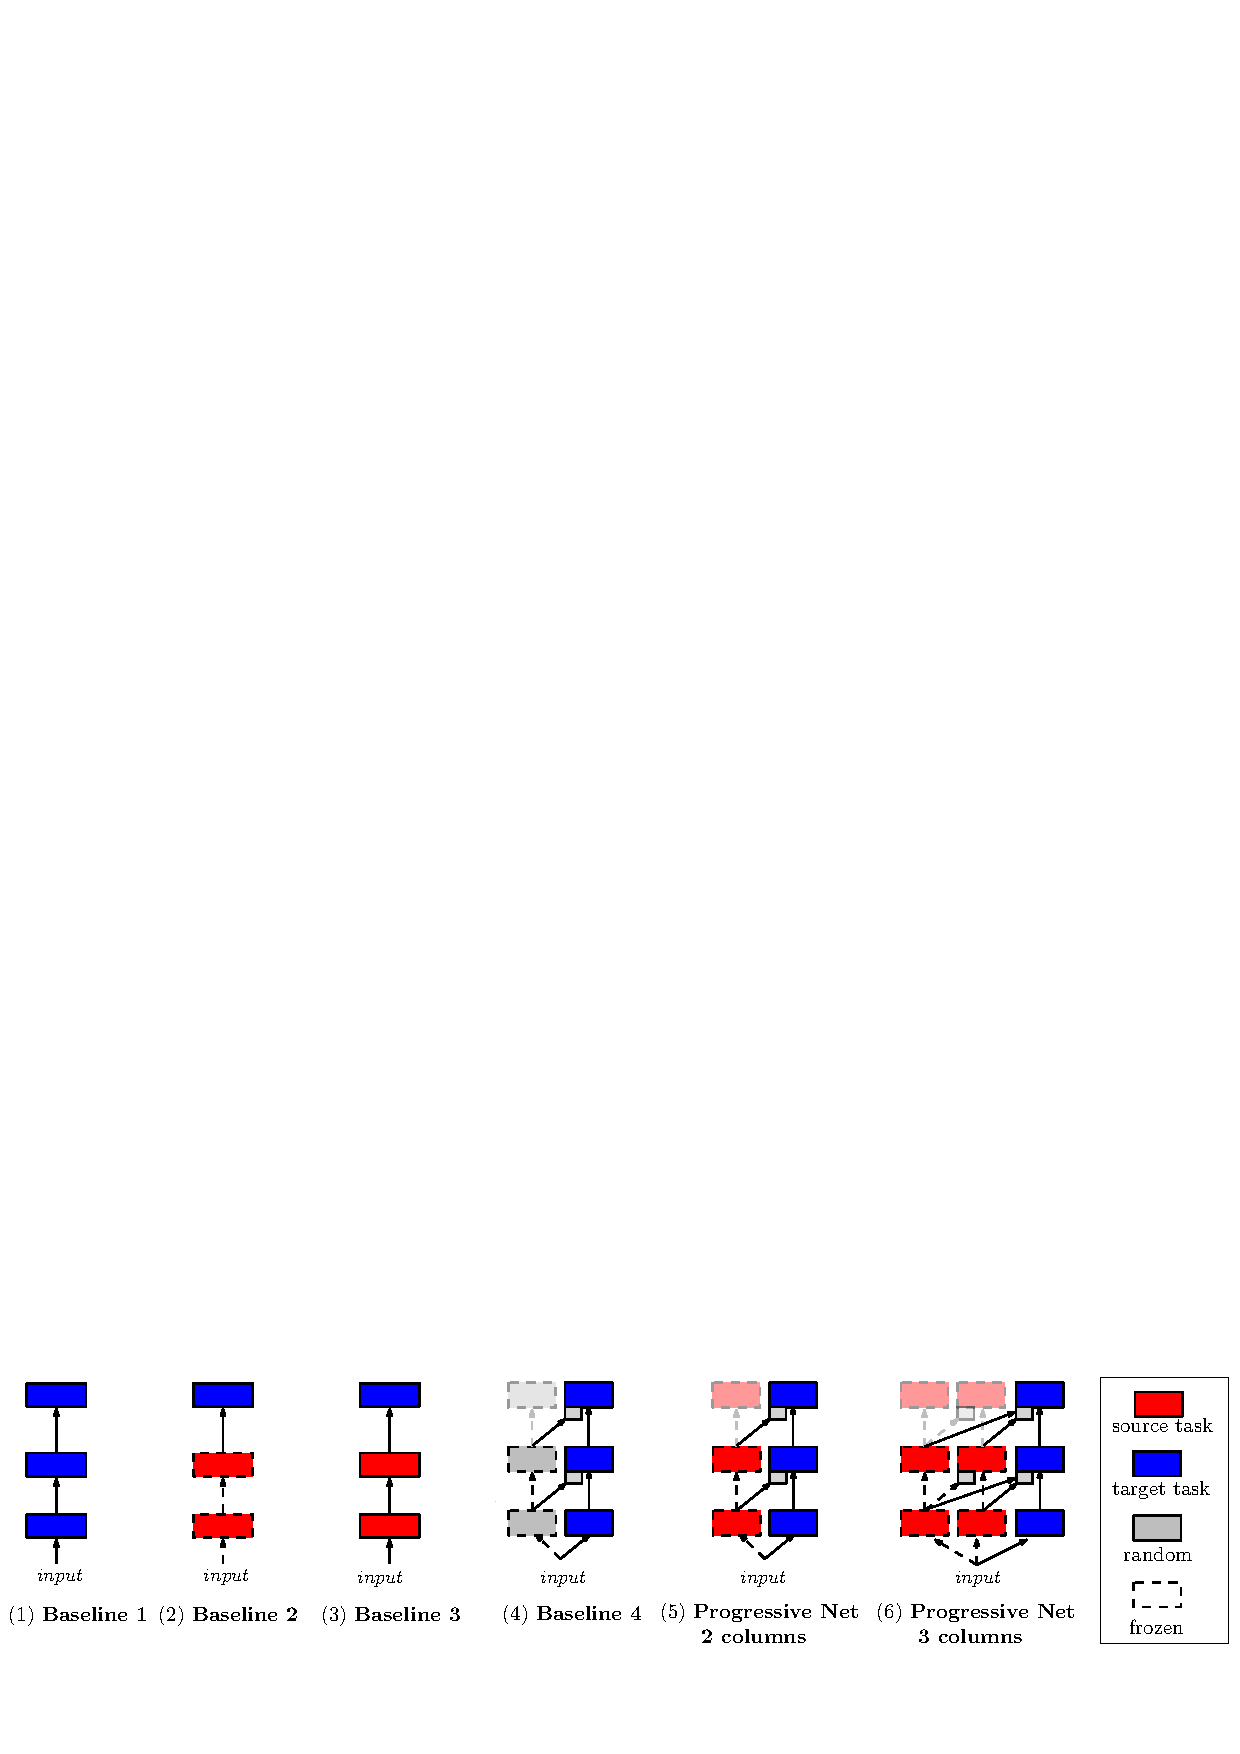
\includegraphics[width=.85\textwidth]{figures/baselineDepiction6}
    \caption{Illustration of different baselines and
      architectures. \emph{Baseline 1} is a single column trained on the target task;
\emph{baseline 2} is a single column, pretrained on a source task and
finetuned on the target task (output layer only); \emph{baseline 3} is
the same as baseline 2 but the whole model is finetuned; and
\emph{baseline 4} is a 2 column progressive architecture,
        with previous column(s) initialized randomly and frozen.
    }
    \label{fig:baselines}
\end{figure}
